\section{Extension A: Hydrogen $n=2$ and the Lamb shift}
The method of Levels 1--4 carries over to a different atom with one new idea: putting two
orbital levels, $2s$ and $2p$, into a single Hamiltonian.

\subsection{Block structure}
The eight $n=2$ states (spin included) are $2S_{1/2}$ (2 states), $2P_{1/2}$ (2) and $2P_{3/2}$ (4).
Both the spin--orbit term and the Zeeman term commute with $\vb{L}^2$, so $l$ is conserved and
\begin{equation}
  H = H(l{=}0) \oplus H(l{=}1).
\end{equation}
Energies are measured from $2P_{1/2}$ at zero field. In the $l=1$ block, $\zeta = \Delta_{2P}/(3/2)$
with $\Delta_{2P} = E(2P_{3/2}) - E(2P_{1/2})$. In the $l=0$ block, $2S_{1/2}$ is raised by the
\emph{Lamb shift} $\Delta_L = E(2S_{1/2}) - E(2P_{1/2})$. The Dirac equation predicts $\Delta_L = 0$;
it is a QED effect, so we take it from experiment ($1057.845\ \si{MHz}$).

\subsection{Consequences}
\begin{enumerate}
  \item \textbf{Weak field.} Each term moves with slope $g_J m_j$, as in Level 2
        ($g_J = 2,\ 2/3,\ 4/3$ for $2S_{1/2},\ 2P_{1/2},\ 2P_{3/2}$).
  \item \textbf{No $2s$--$2p$ mixing by $B$.} Because $l$ is conserved, levels from the two blocks
        \emph{cross} instead of repelling. Mixing them requires an electric field, the basis of the
        Lamb--Retherford experiment (not modelled here).
  \item \textbf{The crossing field measures $\Delta_L$.} The level $2S_{1/2}(m_j{=}-\tfrac12)$
        falls with slope $-g_s/2$ while $2P_{1/2}(m_j{=}+\tfrac12)$ rises with slope $+g_{1/2}/2$. A first-order estimate is
        \begin{equation}
          B_\times \approx \frac{\Delta_L}{\mu_B\,(g_s/2 + g_{1/2}/2)} = 566.5\ \si{G}.
        \end{equation}
        The exact diagonalisation gives $573.4\ \si{G}$: the field also mixes $2P_{1/2}$ with
        $2P_{3/2}$, bending $2P_{1/2}$ down by about $13\ \si{MHz}$ at this field. The literature quotes
        ``about 570 G'' (a study that also includes hyperfine structure, which our model neglects).
        Doubling $\Delta_L$ in the model moves the crossing from $573\ \si{G}$ to $1160\ \si{G}$.
\end{enumerate}

\begin{table}[h]
\centering
\begin{tabular}{lrr}
\toprule
Quantity & Reference & Model \\
\midrule
$2P_{3/2}-2P_{1/2}$ (MHz) & 10969.13 (input; Dirac theory: 10949) & input \\
$2S_{1/2}-2P_{1/2}$ Lamb shift (MHz) & 1057.845 (input) & input \\
$2S_{1/2}(-\tfrac12)\times 2P_{1/2}(+\tfrac12)$ crossing (G) & about 570 & 573.4 \\
\bottomrule
\end{tabular}
\caption{Hydrogen $n=2$. Inputs: Lamb shift $1057.845(9)$ MHz (Lundeen and Pipkin, quoted in \cite{arxiv0809}); fine structure $10969.13(10)$ MHz \cite{baird1972}.}
\end{table}

\begin{figure}[h]
\centering
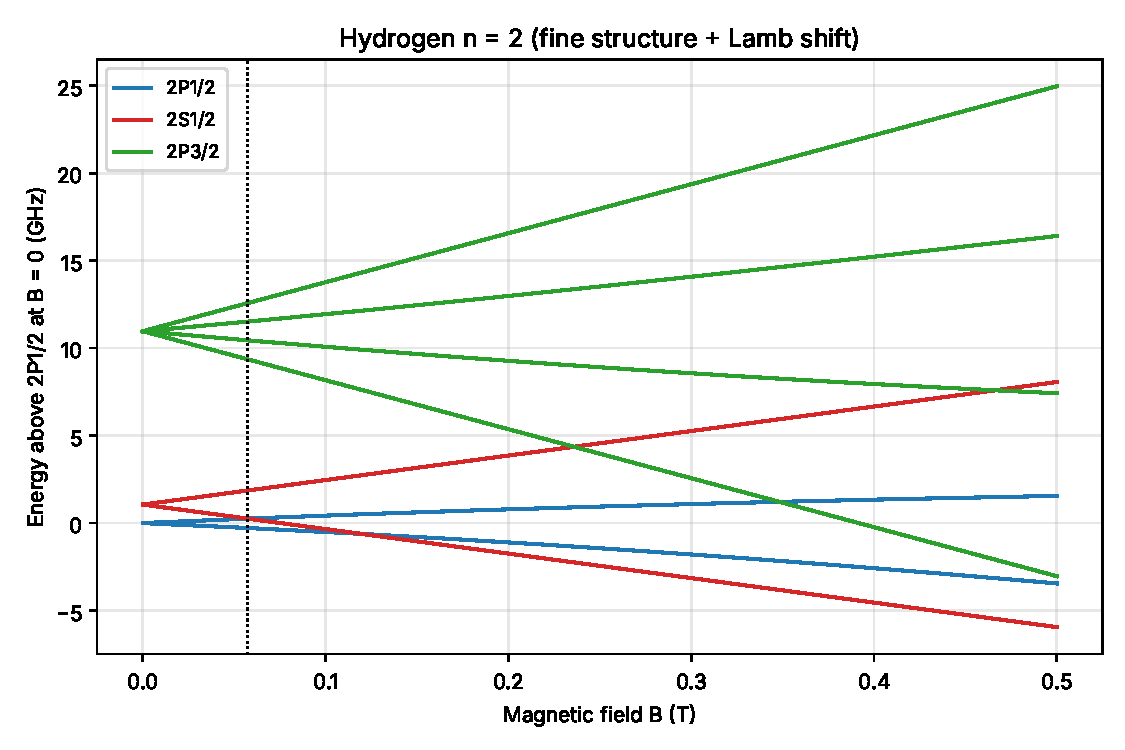
\includegraphics[width=0.8\textwidth]{hydrogen_n2_levels.pdf}
\caption{Hydrogen $n=2$ levels versus magnetic field (red: $2S_{1/2}$, blue: $2P_{1/2}$, green: $2P_{3/2}$).
The dotted line marks the crossing near 570 G.}
\end{figure}
